\documentclass{article}
\usepackage[utf8]{inputenc}
\usepackage{comment}

%%%%%%%%%%%%%%%%%%%%%%% To include python code? %%%%%%%%%%%%%%%%%%%%%%%
\usepackage{color}
\usepackage{listings}
\usepackage{setspace}
\definecolor{Code}{rgb}{0,0,0}
\definecolor{Decorators}{rgb}{0.5,0.5,0.5}
\definecolor{Numbers}{rgb}{0.5,0,0}
\definecolor{MatchingBrackets}{rgb}{0.25,0.5,0.5}
\definecolor{Keywords}{rgb}{0,0,1}
\definecolor{self}{rgb}{0,0,0}
\definecolor{Strings}{rgb}{0,0.63,0}
\definecolor{Comments}{rgb}{0,0.63,1}
\definecolor{Backquotes}{rgb}{0,0,0}
\definecolor{Classname}{rgb}{0,0,0}
\definecolor{FunctionName}{rgb}{0,0,0}
\definecolor{Operators}{rgb}{0,0,0}
\definecolor{Background}{rgb}{0.98,0.98,0.98}
\lstdefinelanguage{Python}{
numbers=left,
numberstyle=\footnotesize,
numbersep=1em,
xleftmargin=1em,
framextopmargin=2em,
framexbottommargin=2em,
showspaces=false,
showtabs=false,
showstringspaces=false,
frame=l,
tabsize=4,
% Basic
basicstyle=\ttfamily\small\setstretch{1},
backgroundcolor=\color{Background},
% Comments
commentstyle=\color{Comments}\slshape,
% Strings
stringstyle=\color{Strings},
morecomment=[s][\color{Strings}]{"""}{"""},
morecomment=[s][\color{Strings}]{'''}{'''},
% keywords
morekeywords={import,from,class,def,for,while,if,is,in,elif,else,not,and,or,print,break,continue,return,True,False,None,access,as,,del,except,exec,finally,global,import,lambda,pass,print,raise,try,assert},
keywordstyle={\color{Keywords}\bfseries},
% additional keywords
morekeywords={[2]@invariant,pylab,numpy,np,scipy},
keywordstyle={[2]\color{Decorators}\slshape},
emph={self},
emphstyle={\color{self}\slshape},
%
}


\usepackage{pdfpages}
\usepackage{graphicx}  % For PNG

% Give Table of Contents Hyperlinks
\usepackage{hyperref}
\hypersetup{
    colorlinks,
    citecolor=black,
    filecolor=black,
    linkcolor=black,
    urlcolor=blue
}
\pagenumbering{gobble}
% \pagenumbering{roman} % set the numbering style to lowercase letter

\title{\textbf{Homework 3}}

\author{MacMillan, Kyle}
\date{October 12, 2018}

\begin{document}


\addcontentsline{toc}{section}{Title}
\maketitle

\newpage
\tableofcontents
\addcontentsline{toc}{section}{Table of Contents}

\pagenumbering{roman}   % Set TOC page numbering to lowercase roman numerals



%%%%%%%%%%%%%%%%%%%%%%%%%%%% INTRO SECTION %%%%%%%%%%%%%%%%%%%%%%%%%%%%
\newpage
\hypersetup{
    colorlinks,
    citecolor=blue,
    filecolor=black,
    linkcolor=blue,
    urlcolor=blue
}
\pagenumbering{arabic}  % Set content page numbering to arabic numerals

\setcounter{page}{1}
\newpage
\section{\textbf{Problem 6.5}}
Figure \ref{fig:6.5.a} shows the required plot.

\begin{figure}[htbp]
  \centering
  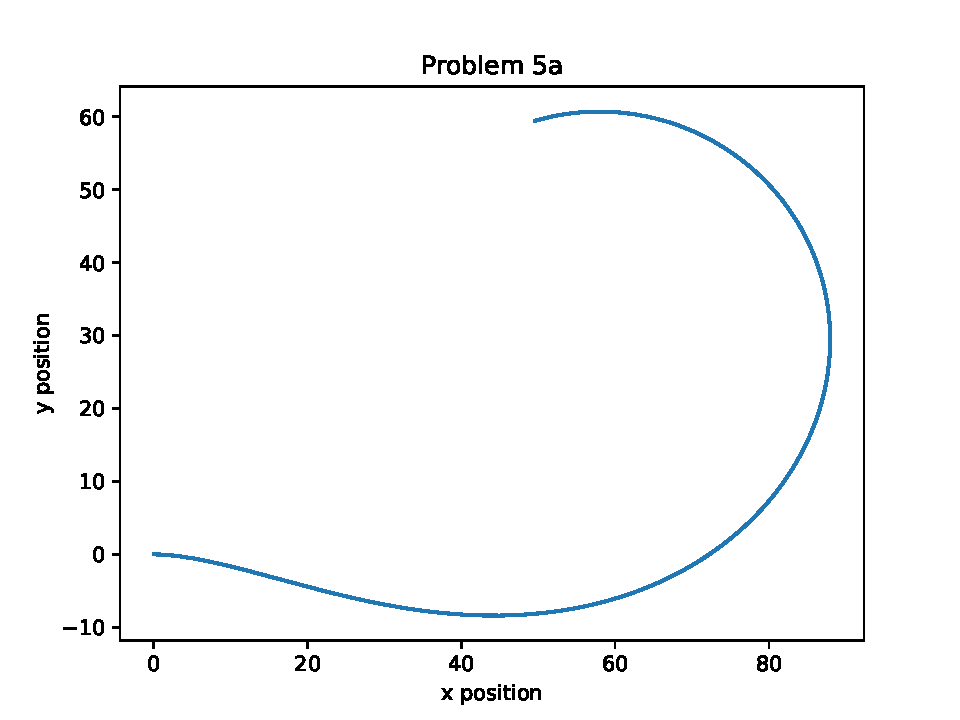
\includepdf[pages={1}]{p6-5-a.pdf}
  \caption{Problem 6.5.a}
  \label{fig:6.5.a}
\end{figure}


Figure \ref{fig:6.5.b} shows the data points that were saved.

\begin{figure}[htbp]
  \centering
  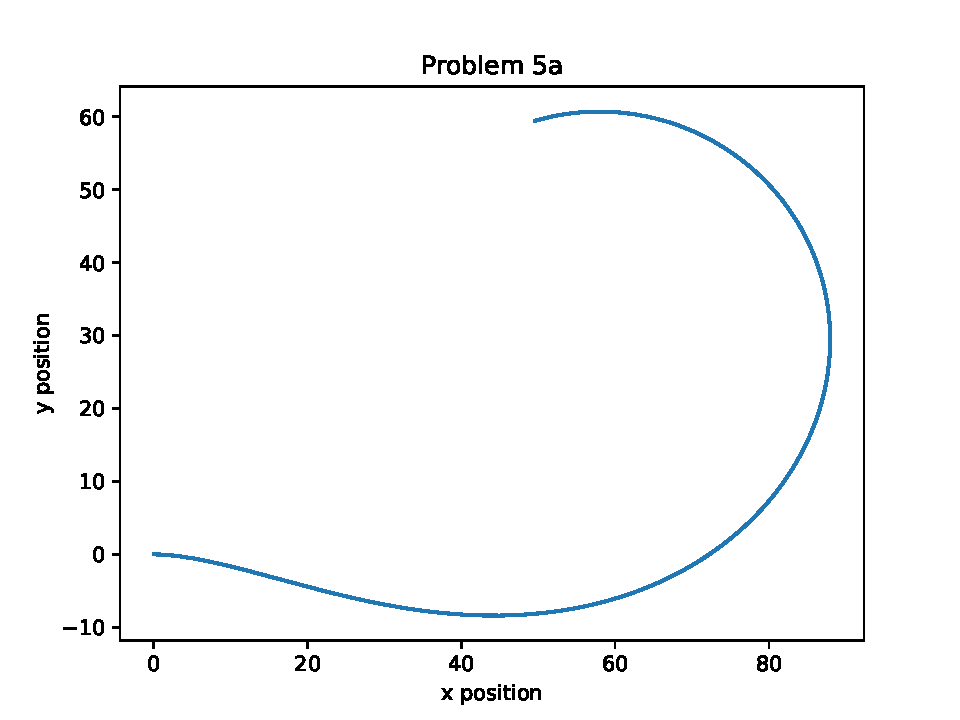
\includepdf[pages={1}]{p6-5-b.pdf}
  \caption{Problem 6.5.b}
  \label{fig:6.5.b}
\end{figure}


Figure \ref{fig:6.5.c} shows the data points that were saved.

\begin{figure}[htbp]
  \centering
  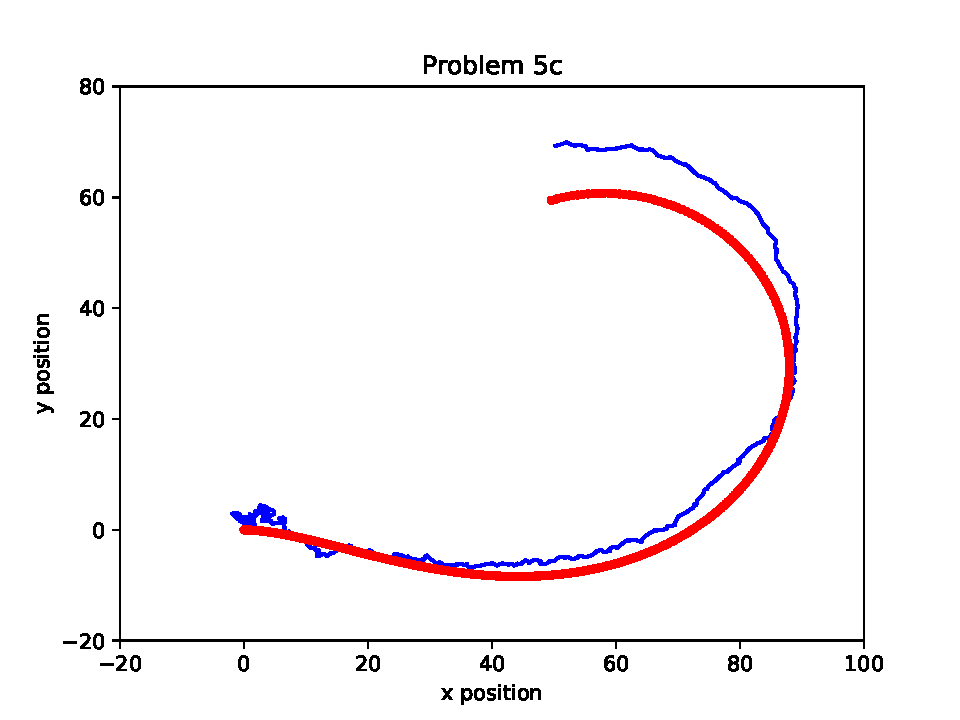
\includepdf[pages={1}]{p6-5-c.pdf}
  \caption{Problem 6.5.c}
  \label{fig:6.5.c}
\end{figure}


Figure \ref{fig:6.5.d} shows the data points that were saved.

\begin{figure}[htbp]
  \centering
  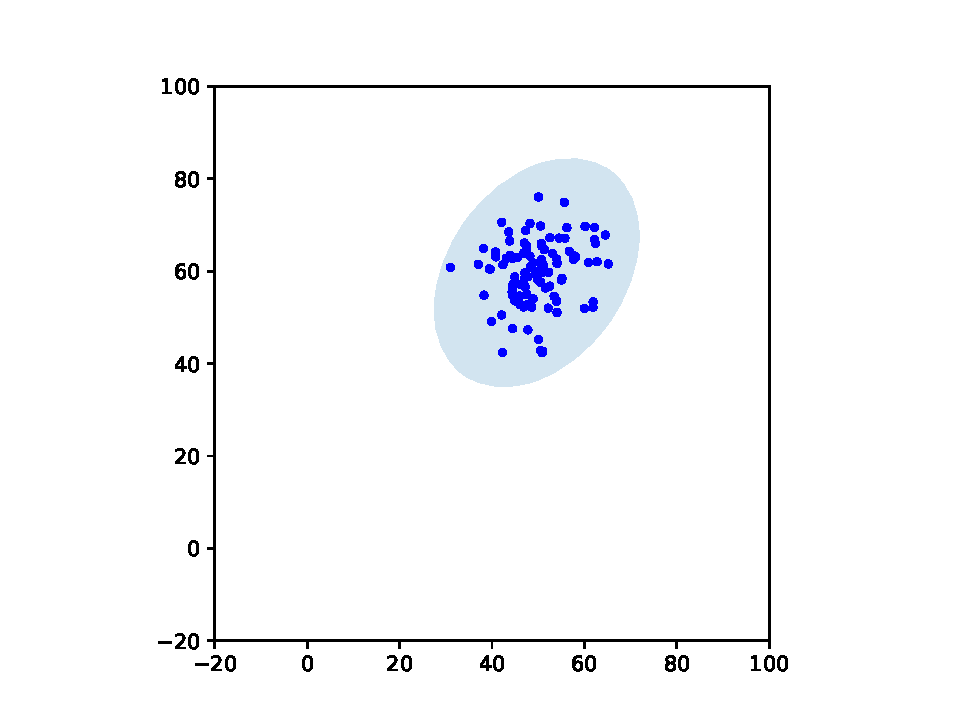
\includepdf[pages={1}]{p6-5-d.pdf}
  \caption{Problem 6.5.d}
  \label{fig:6.5.d}
\end{figure}


\section{\textbf{Problem 6.8}}


\end{document}
